\documentclass[handout]{beamer}
\usepackage{amsmath,amssymb,amsthm}
\usepackage[utf8]{inputenc}
\usepackage[russian]{babel}
\usepackage{graphicx}
\usepackage{subcaption}
\usetheme{Boadilla}


\title{Научно-исследовательская практика}
\subtitle{Четыре в ряд}
\author[Четыре в ряд]{Толпекин Максим Александрович\\Тарасов Егор Александрович}
\institute[]{Институт физико-математических наук и информационных технологий БФУ им. И. Канта}
\date{1 июля 2022 года}

\setbeamertemplate{caption}[numbered]

\newtheorem*{myproblem}{Цель игры}
\newtheorem*{modules}{Модули}
\newtheorem*{mathre}{}
\newtheorem*{minimax}{Минимакс}
\newtheorem*{alphab}{Альфа-бета-отсечение}
\begin{document}
	
	\section{Титульный лист}
	\begin{frame}
		\titlepage
	\end{frame}
	
	\section{Описание механики игры}
	\begin{frame}{Описание механики игры}
		\begin{myproblem}
		  Цель игры — расположить раньше противника подряд по горизонтали, вертикали или диагонали четыре фишки своего цвета.
		\end{myproblem}
		\begin{figure}
		  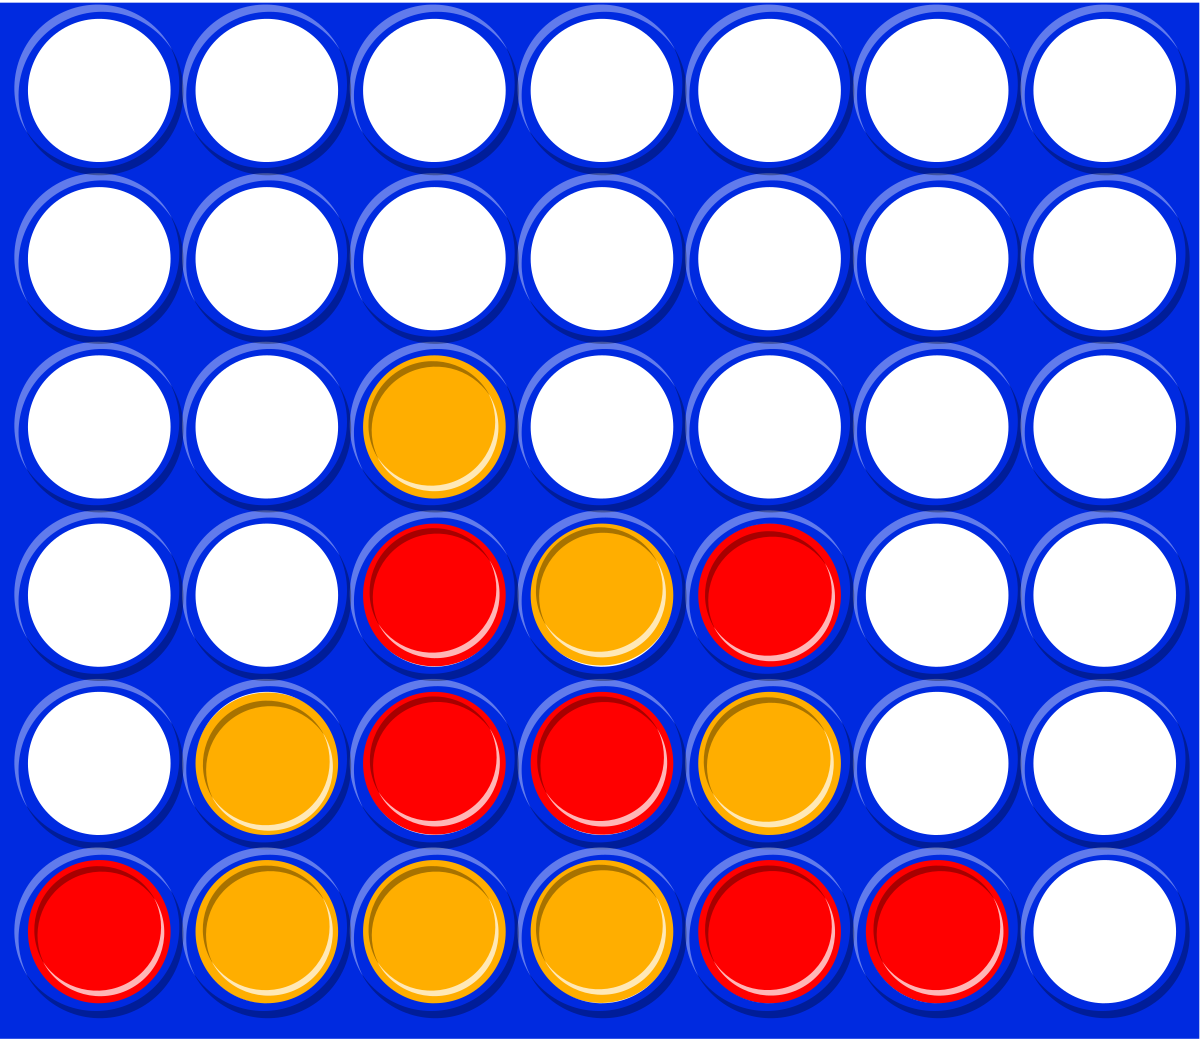
\includegraphics[width=0.5\linewidth]{4r.png}
		  \caption{Четыре в ряд}
	    \end{figure}
	\end{frame}

    \section{Математическое решение}
    \begin{frame}{Математическое решение}
    	\begin{mathre}
    	Математически игра была решена Джеймсом Д. Алленом  1 октября 1988, а также независимо Виктором Аллисом 16 октября 1988.\\[2mm]
    	Роняя первую фишку в колонку посередине, первый игрок может обеспечить себе выигрыш. Роняя первую фишку в одну из соседних колонок, первый игрок позволяет противнику сыграть вничью. Начиная игру с одной из четырёх крайних колонок, первый игрок позволяет выиграть противнику.
    	\end{mathre}
    \end{frame}

	
	\section{Описание реализации}
	\begin{frame}{Описание реализации}

	\begin{modules}
		\begin{enumerate}
		 \item NumPy
		 \item Pygame
		 \item sys
		 \item math
		\end{enumerate}
	\end{modules}

	\end{frame}

	\section{Минимакс}
    \begin{frame}{Алгоритм минимакс}
		\begin{figure}[h!]
			\centering
			\begin{subfigure}[b]{0.49\linewidth}
				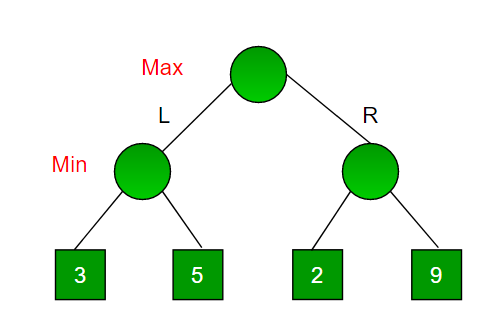
\includegraphics[width=1\linewidth]{minmax.png}
				\caption{Начальное состояние графа}
			\end{subfigure}
			\begin{subfigure}[b]{0.49\linewidth}
				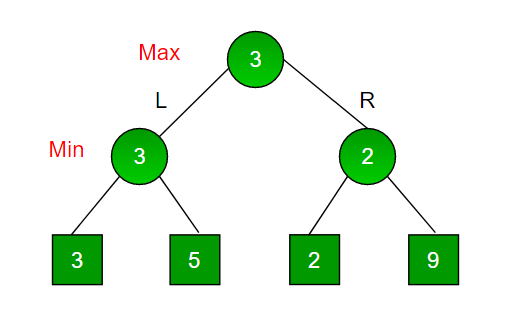
\includegraphics[width=1\linewidth]{minmax1.png}
				\caption{Конечное состояние графа}
			\end{subfigure}
		  \caption{Алгоритм минимакс}
		\end{figure}
    \end{frame}	

	\section{Альфа-бета-отсечение}
    \begin{frame}{Альфа-бета-отсечение}
    	\begin{figure}
    		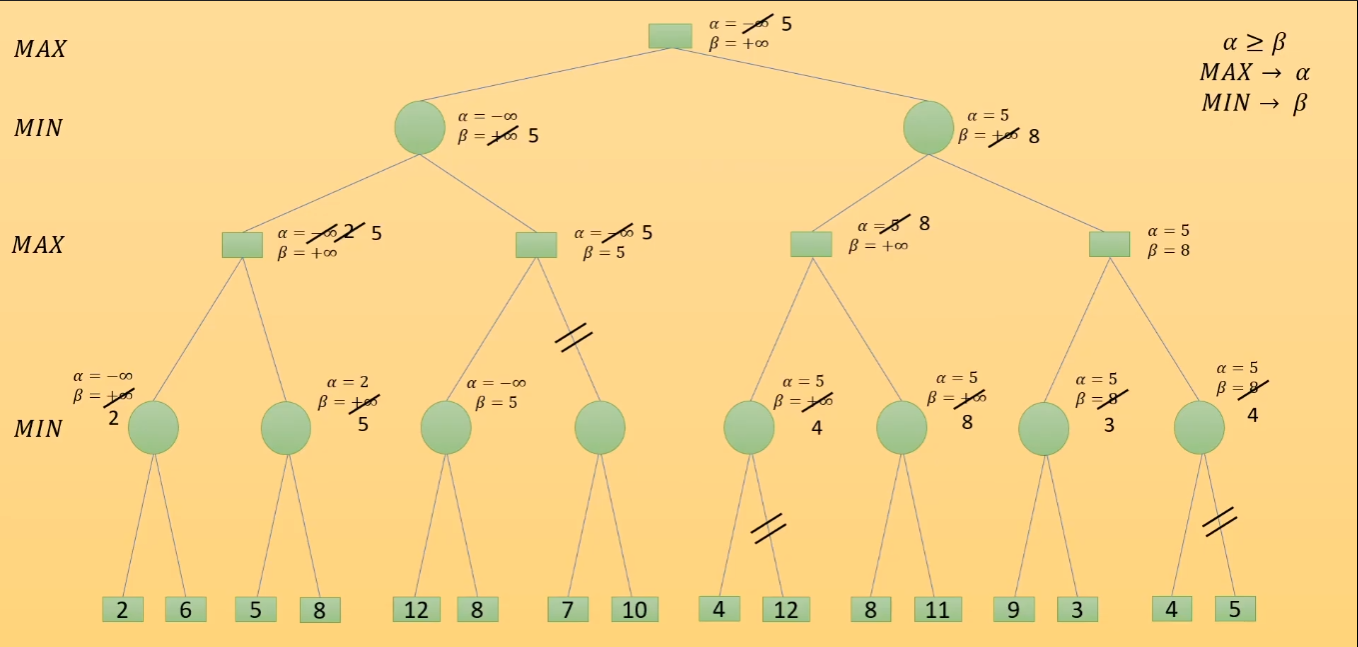
\includegraphics[width=0.9\linewidth]{unknown.png}
    		\caption{Пример Альфа-бета-отсечения}
    	\end{figure}
    \end{frame}
	
	\section{Демонстрация решения}
	\begin{frame}{Он-лайн демонстрация кода и его работы}
		Сейчас мы продемонсрируем работу нашей игры!\centering		
	\end{frame}
	
	
	\section{Заключение}
	\begin{frame}{Заключение}
		 В этой научно-исследовательской работе мы потренировались в создании кода для небольших игр, в частности, для игры четыре в ряд. А так же мы рассмотрели новые алгоритмы которые используются в теории игр.
		
	\end{frame}
	
\end{document}